\section{Numerik und Durchführung} % (fold)
\label{sec:numerik_und_durchf_hrung}

	\subsection{Räumliche Diskretisierung und Gitter} % (fold)
	\label{sub:r_umliche_diskretisierung_und_gitter}
	
		Die Simulation findet im rechteckigen Gebiert $\Omega:= [0,a]\times [0,b] \subset \SR^2$ statt.
		Dieses wird in $i_{max} \cdot j_{max}$ rechteckige Zellen zerlegt.
		Die Zellen des räumlichen Gitters besitzen die Maße $\delta x \cdot \delta y$  wobei gilt:

		\[ \delta x := \frac{a}{i_{max}} \qquad \text{und} \qquad \delta y := \frac{b}{j_{max}}\]

		Die skalaren Felder $u$, $v$, und $p$ ordnen wir auf diesem Gitter wie in Abbildung \ref{fig:VerschGitter} zu sehen an.

		\begin{figure}[h]
			\center
			\fbox{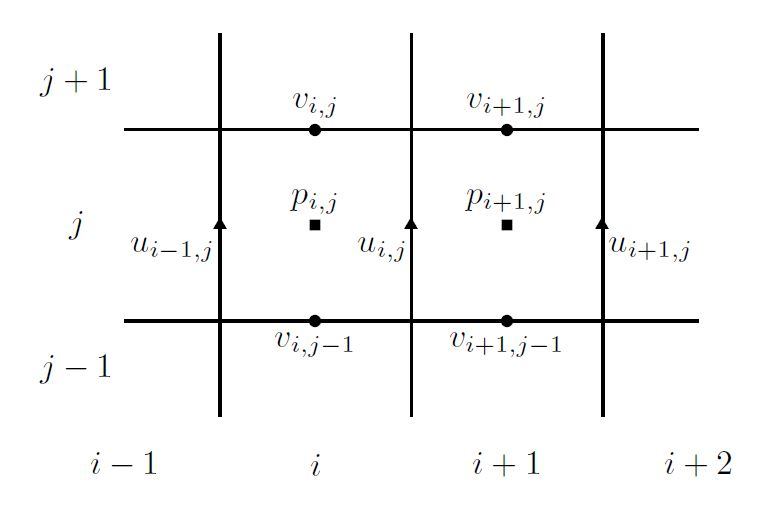
\includegraphics[scale=0.5]{VerschGitter.JPG}}
			\caption{Schema für die Position der Geschwindigkeitskomponenten $u$, $v$ sowie des Drucks $p$ auf dem Gitter \\ Quelle: \cite{nsfd} }
			\label{fig:VerschGitter}
		\end{figure}

		Durch die verschobenen Gitter lassen sich mögliche Oszillationen und Uneindeutigkeiten des Drucks verhindern.
		Die grauen Zellen in Abbildung \ref{fig:Randzellen} bilden die Randzellen, sie erhalten bei Initialisierung des Programms feste Werte entsprechend den jeweiligen Randwertproblemen und behalten diese während der gesamten Simulation bei.

		\begin{figure}[h]
			\center
			\fbox{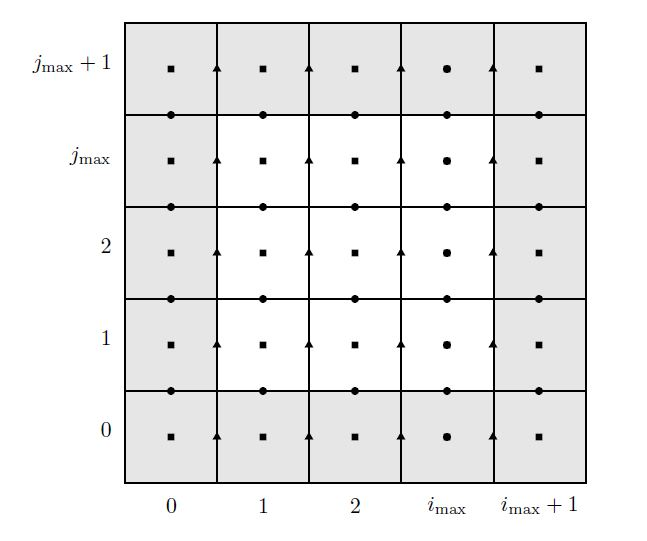
\includegraphics[scale=0.5]{Randzellen.JPG}}
			\caption{Darstellung der Randzellen mit den entsprechenden Randbedingungen \\ Quelle: \cite{nsfd} }
			\label{fig:Randzellen}
		\end{figure}

	% subsection r_umliche_diskretisierung_und_gitter (end)


	\subsection{Lösen der Impulsgleichungen} % (fold)
	\label{sub:l_sen_der_impulsgleichungen}

		Die Variablen werden zum Zeitpunkt $n$ betrachtet, die nachfolgenden Geschwindigkeitskomponenten werden mit Hilfe eines einfachen Euler-Vorwärts-Schrittes berechnet:

		\[ u^{(n+1)} = F^{(n)} - \delta t \frac{\partial p^{(n+1)}}{\partial x} \]

		\[ v^{(n+1)} = G^{(n)} - \delta t \frac{\partial p^{(n+1)}}{\partial y} \]

		Dabei sind die Funktionen $F$ und $G$ wie folgt definiert:

		\[ F = u + \delta t \boxb{ \frac{1}{Re} \curvb{ \frac{\partial ^{2} u}{\partial x ^{2}} + \frac{\partial ^{2} u}{\partial y ^{2}}} 
		- \frac{ \partial (u^{2}) }{ \partial x} - \frac{ \partial (uv) }{ \partial y} + g_x } \]

		\[ G = v + \delta t \boxb{ \frac{1}{Re} \curvb{ \frac{\partial ^{2} v}{\partial x ^{2}} + \frac{\partial ^{2} v}{\partial y ^{2}}} 
		- \frac{ \partial (uv) }{ \partial x} - \frac{ \partial (v^{2}) }{ \partial y} + g_y } \]

		Das Verfahren ist wie wir sehen expliziet in den Geschwindigkeitskomponenten und impliziet im Druck.
		Die Druckberechnung wird unter Abschnitt \ref{sub:berechnung_des_drucks} genauer beschreiben.
		Der Zeitschritt $\delta t$ muss sorgfältig gewählt werden, um die Stabilität der Simulation zu gewährleisten.
		Nach Griebel, Dornseifer und Neuhöfer sollte er wie folgendermaßen gewählt werden:

		\[ \delta t := \tau \min \curvb{ \frac{Re}{2} \frac{1}{\delta x^{-2} + \delta y^{-2}} , \frac{\delta x}{\abs{u_{max}}} , 
		\frac{\delta y}{\abs{v_{max}}} } \]

		Hierbei ist $\tau$ ein Sicherheitsfaktor zwischen 0 und 1.
		Im Programm wird er meist auf 0.5 gesetzt.

	
	% subsection l_sen_der_impulsgleichungen (end)

	\subsection{Ableitungs - Stencils} % (fold)
	\label{sub:ableitungs_stencils}
	
		Die Ableitungen werden mit Hilfe der Finiten-Differenzen-Methode berechnet.
		Dabei werden die ersten Ortsableitungen beispielsweise des Drucks durch den einfachen rechtseitigen Differenzenquotienten approximiert.

		\[ \boxb{\frac{\partial p}{\partial x}}_{i,j} = \frac{p_{i+1,j} - p_{i,j}}{\delta x}, \qquad 
		\boxb{\frac{\partial p}{\partial y}}_{i,j} = \frac{p_{i,j+1} - p_{i,j}}{\delta y} \]

		Für die zweiten Ableitungen werden standardmäßig zentrierte Differenzen verwendet.

		\[ \boxb{\frac{\partial ^2 u}{\partial x ^2}}_{i,j} = \frac{u_{i+1,j} - 2 u_{i,j} + u_{i-1,j}}{(\delta x) ^2}, \qquad 
		\boxb{\frac{\partial ^2 u}{\partial y ^2}}_{i,j} = \frac{u_{i,j+1} - 2 u_{i,j} + u_{i,j-1}}{(\delta y) ^2} \]

		Analoge Vorschriften liegen für die Ableitungen von $v$ vor.
		Die Ableitungen der gemischten und nichtlinearen Terme werden durch eine Linearkombination von zentrierten Differenzen und Donor-Cell-Stencils ermittelt.

		\begin{alignat*}{3}
			\boxb{ \frac{\partial (u ^2)}{\partial x} }_{i,j} &= \frac{1}{4 \delta x}
			\curvb{ (u_{i,j} + u_{i+1,j})^2 - (u_{i-1,j} + u_{i,j})^2 } \\
			&+ \gamma \frac{1}{4 \delta x} 
			\curvb{ \abs{u_{i,j} + u_{i+1,j}} (u_{i,j} - u_{i+1,j}) - \abs{u_{i-1,j} + u_{i,j}} (u_{i-1,j} - u_{i,j}) } \\
			\boxb{ \frac{\partial (v ^2)}{\partial y} }_{i,j} &= \frac{1}{4 \delta y}
			\curvb{ (v_{i,j} + v_{i,j+1})^2 - (v_{i,j-1} + v_{i,j})^2 } \\
			&+ \gamma \frac{1}{4 \delta y} 
			\curvb{ \abs{v_{i,j} + v_{i,j+1}} (v_{i,j} - u_{i,j+1}) - \abs{v_{i,j-1} + v_{i,j}} (v_{i,j-1} - v_{i,j}) } \\
			\boxb{ \frac{\partial (uv)}{\partial x} }_{i,j} &= \frac{1}{4 \delta x}
			\curvb{ (u_{i,j} + u_{i,j+1})(v_{i,j} + v_{i+1,j}) - (u_{i-1,j} + u_{i-1,j+1})(v_{i-1,j} + v_{i,j}) } \\
			&+ \gamma \frac{1}{4 \delta x} 
			\curvb{ \abs{u_{i,j} + u_{i,j+1}} (v_{i,j} - v_{i+1,j}) - \abs{u_{i-1,j} + u_{i-1,j+1}} (v_{i-1,j} - v_{i,j}) } \\
			\boxb{ \frac{\partial (uv)}{\partial y} }_{i,j} &= \frac{1}{4 \delta y}
			\curvb{ (u_{i,j} + u_{i,j+1})(v_{i,j} + v_{i+1,j}) - (u_{i,j-1} + u_{i,j})(v_{i,j-1} + v_{i+1,j-1}) } \\
			&+ \gamma \frac{1}{4 \delta y} 
			\curvb{ \abs{v_{i,j} + v_{i+1,j}} (u_{i,j} - u_{i,j+1}) - \abs{v_{i,j-1} + v_{i+1,j-1}} (u_{i,j-1} - u_{i,j}) } \\
		\end{alignat*}

		Der Vorfaktor $\gamma$ gewichtet hierbei die Anteile von zentrierten Differenzen und Donor-Cell-Stencils.
		Er sollte nach Hirt so gewählt werden, dass er folgende Bedingung erfüllt:

		\[ \gamma \geq \max_{ij} \curvb{ \frac{\abs{u_{i,j}} \delta t}{\delta x} , \frac{\abs{v_{i,j}} \delta t}{\delta y} } \]

		Jedoch wird er in unserem Programm zu Beginn auf einen konstanten Wert gesetzt, wie er auch in anderen Simulationen bereits verwendet wurde.

	% subsection ableitungs_stencils (end)


	\subsection{Berechnung des Drucks} % (fold)
	\label{sub:berechnung_des_drucks}

		Zur Bestimmung des Drucks verwenden wir die Kontinuitätsgleichung.

		\[ \frac{\partial u^{n+1}}{\partial x} + \frac{\partial v^{n+1}}{\partial y} = 0\]

		Zusammen mit der unter \ref{sub:l_sen_der_impulsgleichungen} angegebenen Gleichung für die Ermittlung der Geschwindigkeiten lässt sich folgende Poisson-Gleichung für den Druck ableiten:

		\[ \frac{\partial ^{2} p^{(n+1)}}{\partial x^{2}} + \frac{\partial ^{2} p^{(n+1)}}{\partial y^{2}} = 
		\frac{1}{\delta t} \curvb{ \frac{\partial F^{(n)}}{\partial x} + \frac{\partial G^{(n)}}{\partial y} } \]

		Die zweiten und ersten Ortsableituungen werden analog zu den unter \ref{sub:ableitungs_stencils} beschriebenen Ableitungen gebildet.
		Zum lösen der diskreten Poissongleichung wird hier das Successive-Over-Relaxation Verfahren (SOR) angewendet.
		Bei diesem iterativen Verfahren setzen wir den Startwert zu $p_{i,j} ^{(n)}$, jeder weitere Iterationsschritt ergibt sich dann zu:

		\[ p_{i,j} ^{it+1} = (1- \omega) p_{i,j}^{it} + \frac{\omega}{2 (\delta x)^{-2} + 2 (\delta y)^{-2}} 
		\curvb{ \frac{ p_{i+1,j}^{it} + p_{i-1,j}^{it+1} }{(\delta x)^2} + \frac{ p_{i,j+1}^{it} + p_{i,j-1}^{it+1} }{(\delta y)^2} - \text{RHS}_{i,j} } \]

		Wobei RHS die rechte Seite der Poissongleichung bezeichnet.
		In jeder Iteration wird das Residuum $r$ berechnet 

		\[ r_{i,j}^{it+1} = \frac{ p_{i+1,j}^{it+1} - 2 p_{i,j}^{it+1} + p_{i-1,j}^{it+1} }{ (\delta x)^2 } + 
		\frac{ p_{i,j+1}^{it+1} - 2 p_{i,j}^{it+1} + p_{i,j-1}^{it+1} }{ (\delta y)^2 } - \text{RHS}_{i,j}\]

		bis die Norm des Residuuums eine vorgegebene relative Toleranzgrenze unterschreitet.

		\[ \norm{r^{it+1}} < \epsilon \norm{p^{it}} \]

		Wobei die Norm im Versuch durch die Maximumsnorm gebildet wird und $\epsilon$ eine festgelegte kleine Konstante darstellt.
		Die Randzellen werden bei jedem Iterationsschritt einfach durch Kopieren der jeweiligen Nachbarzellen gefüllt.


	% subsection berechnung_des_drucks (end)

% section numerik_und_durchf_hrung (end) 